\documentclass[11pt]{amsbook}

\usepackage{../HBSuerDemir}

\begin{document}

    \hPage{b2p1/118}
    
    A vector having coincident end points or having a zero length is the \underline{zero vector} denoted by $\vec{PP}$ or $\vec{0}$ or simply 0 with indefinite direction and sense.
    
    Vectors may as well be denoted by single letters with an arrow on top: $\vec{a},\vec{u},\vec{e}$.
    
    \underline{Equality:}
    
    Two vectors $\vec{AB},\vec{CD}$ having to same direction, the same sense and the same length are considered \underline{equal}, written $\vec{AB}=\vec{CD}$. \\
    
    \qquad If $\vec{AB} = \vec{CD}$ then ABCD is a parallelogram (which may be
    
    \begin{minipage}{0.6\textwidth}
    degenerate one) and one of these vectors can be obtained from the other by a translation (under which direction, sense and length are preserved).
	\end{minipage}
	\hfill
	\begin{minipage}{0.4\textwidth}
	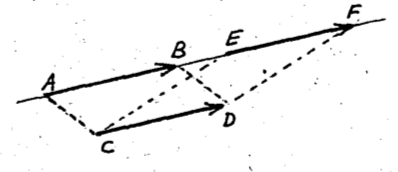
\includegraphics[width=\textwidth]{images/b2p1-118-fig01.png}
	\end{minipage}
    
    In the figure, ABCD and CDFE are parallelograms.It follows that $\vec{AB}=\vec{CD}=\vec{EF}$. Note that ABFE is a degenerate parallelogram. 
    
    From this definition, vectors can always be drawn to have the same initial point.
    
    Two vectors are unequal if they differ from each other either in direction or in sense or in length.
    
    A vector with fixed initial point is a \underline{bound vector} (or a \underline{position vector}), one restricted to lie on a fixed line is a \underline{sliding vector} and ones with no such restrictions are \underline{free vectors}.
    
    A free vector remains invariant under any translation, while a sliding vector remains invariant under a translation in the direction of vector.

\end{document}  
